\documentclass{amsart}

\usepackage{amssymb, amsfonts, hyperref, graphicx, bbm}
\usepackage{enumerate}

\newtheorem{thm}{Theorem}[section]
\newtheorem{cor}[thm]{Corollary}
\newtheorem{prop}[thm]{Proposition}
\newtheorem{lem}[thm]{Lemma}

\theoremstyle{definition}
\newtheorem{defn}[thm]{Definition}
\newtheorem{defns}[thm]{Definitions}
\newtheorem{con}[thm]{Construction}
\newtheorem{exmp}[thm]{Example}
\newtheorem{exmps}[thm]{Examples}
\newtheorem{notn}[thm]{Notation}
\newtheorem{notns}[thm]{Notations}
\newtheorem{addm}[thm]{Addendum}
\newtheorem{exer}[thm]{Exercise}

\theoremstyle{remark}
\newtheorem{rem}[thm]{Remark}
\newtheorem{rems}[thm]{Remarks}
\newtheorem{warn}[thm]{Warning}
\newtheorem{sch}[thm]{Scholium}

\bibliographystyle{plain}

\graphicspath{ {../figures/} }

%--------Meta Data: Fill in your info------
\title{Optimizing Multistage Portfolio Returns with Risk Constraints}

\author{Kurt Ehlert}

\date{\today}

\begin{document}

\maketitle

\tableofcontents

\section{Modeling Stocks with Geometric Brownian Motion}
Stochastic differential equations (SDEs) are commonly used to model stock prices over time. In particular,
geometric Brownian motion (GBM) is often used.\cite{hull} In this paper, we will use GBM with constant coefficients to model stock prices over time. The SDE for GBM is
\begin{equation}\label{eq:GBM_SDE}
dX_t = \mu X_t dt + \sigma X_t dB_t
\end{equation}
where $\mu$ and $\sigma$ are respectively the drift and volatility parameters, and $B_t$ is Brownian motion at time $t$. We call $X_t$ GBM, and see figure \ref{fig:mesh1} for some example GBM paths.

\begin{figure}
\centering
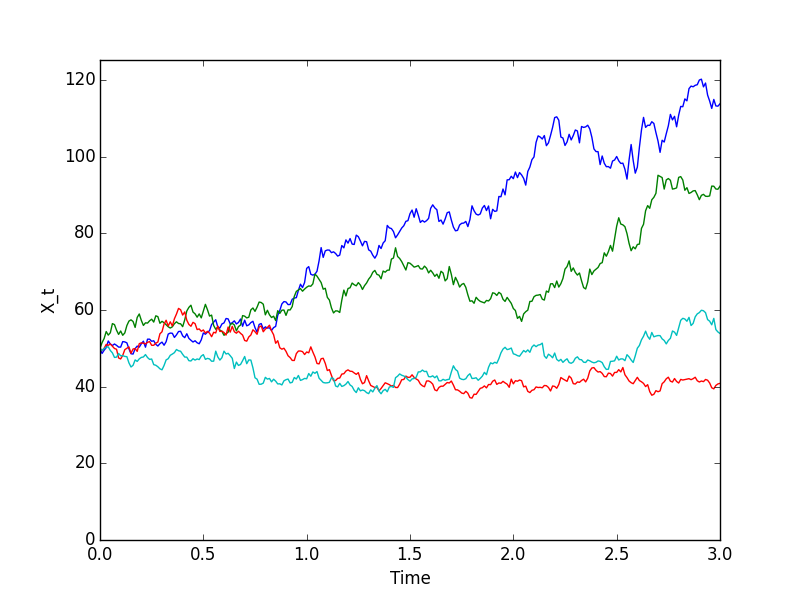
\includegraphics[scale=0.5]{geometric_bm.png}
\caption{Paths of geometric Brownian motion generated by the Euler-Maruyama method. Code is attached (``geometric\_bm.py''). $X_0 = 50, \mu=0.1, \sigma=0.2$.}
\label{fig:mesh1}
\end{figure}

\subsection{1-D Geometric Brownian Motion}
We can solve \eqref{eq:GBM_SDE} by using an integrating factor $Z_t$ \cite[p. 235]{timo}:
\begin{equation*}
Z_t = \exp\left(-\mu t -\sigma B_t + \sigma^2 t/2 \right)
\end{equation*}
For most of the following calculations, we will drop the subscript $t$. By It\^o's lemma we know that
\begin{equation}\label{eq:GBM_SDE_PROD}
d(XZ) = X dZ + Z dX + d[X,Z]
\end{equation}
where $[\cdot,\cdot]$ denotes quadratic covariation. The goal is to substitute in expressions for each of the variables on the right-hand side of the above expression. It\^o's lemma gives us $dZ$
\begin{equation*}
dZ = Z \left[\left(-u + \sigma^2\right) dt - \sigma dB\right]
\end{equation*}
Now we need to calculate the quadratic covariation of $X$ and $Z$,
\begin{align*}
\begin{split}
d[X,Z]_t &= d\left[\int_0^t \mu X_s ds + \int_0^t \sigma X_s dB_s,  \int_0^t (-\mu +\sigma^2) Z_s ds - \int_0^t \sigma Z_s dB_s \right]_t\\
&= d\left[\int_0^t \sigma X_s dB_s,  - \int_0^t \sigma Z_s dB_s \right]_t\\
&= -\sigma ^2 \frac{d}{dt}\int_0^t X_s Z_s ds\\
&= -\sigma^2 X_t Z_t dt
\end{split}
\end{align*}
Thus \eqref{eq:GBM_SDE_PROD} becomes
\begin{align*}
d(XZ) &= Z(\mu X dt + \sigma X dB) + XZ\left[\left(-\mu + \sigma^2 \right)dt -\sigma dB \right] - \sigma^2 X Z dt
&= 0
\end{align*}
Therefore $X_t Z_t = X_0 Z_0 = X_0$, which implies that
\begin{equation}\label{eq:GBM_soln}
X_t =  X_0 Z_t^{-1} = X_0 \exp\left[(\mu - \sigma^2/2) t + \sigma B_t\right]
\end{equation}
Then use It\^o's lemma to check that \eqref{eq:GBM_soln} solves \eqref{eq:GBM_SDE}. It is clear that $\log(X)$ is normally distributed, and
\begin{align*}
\mathbb{E}[\log X ] &= (\mu - \sigma^2/2)t\\
\text{Var}(\log X ) &= \sigma^2 t
\end{align*} 
Thus $X_t$ has a log-normal distribution, and
\begin{align*}
\mathbb{E} X&= X_0 e^\mu\\
\text{Var}X &= X_0^2 e^{2\mu t}(e^{\sigma^2 t} - 1)
\end{align*}

\subsection{Correlated d-Dimensional Geometric Brownian Motion}\label{corr_gmb}
If the Brownian motions driving each SDE are all independent, then the solution is just the d-dimensional version of \eqref{eq:GBM_soln}. The much more interesting case is when there is a correlation between the different dimensions. In other words, we want to find and solve the SDE where $X(t)$ is d-dimensional GBM and $\text{Corr}(\log X_i(t), \log X_j(t)) = \rho_{ij}$. This would allow us to model correlated stock returns. We are interested in the log of the prices, because we want the returns to be correlated. We are not interested in whether or not the stock prices are correlated. In fact, the correlation between the prices goes to zero as times goes to infinity, even if the returns have a positive correlation that's less than one.

The return of stock $i$, $R_i(t)$, is equal to
\begin{equation*}
R_i(t) = \log \frac{X_i(t)}{X_i(0)} = (\mu_i-\sigma_i^2/2)t +\sigma_i dB_i(t)
\end{equation*}
If Corr$(B_i(t),B_j(t)) = \rho_{ij}$, then
\begin{equation*}
\text{Corr}(R_i(t),R_j(t)) = \rho_{ij}
\end{equation*}
Therefore, if we can construct $d$-dimensional Brownian motion that has correlation matrix $\Sigma$, where $(\Sigma)_{ij} = \rho_{ij}$, then we are done. Suppose we can choose $\alpha_{ij}$ such that
\begin{align*}
\sum_{k=1}^i \alpha_{ik}^2 &= 1, \text{ where } 1\le i\le d\\
\sum_{k=1}^i \alpha_{ik}\alpha_{jk}&= \rho_{ij}, \forall j < i \le d
\end{align*}
In other words, we need to find a $d\times d$ lower-triangular matrix $L$, where
\begin{equation*}
L= \begin{bmatrix}
    \alpha_{11} & 0 & 0 & \dots  & 0 \\
    \alpha_{21} & \alpha_{22} & 0 & \dots  & 0 \\
    \vdots & \vdots & \vdots & \ddots & \vdots \\
    \alpha_{d1} & \alpha_{d2} & \alpha_{d3}& \dots  & \alpha_{dd}
\end{bmatrix}
\end{equation*}
such that
\begin{equation*}
L L^T = \Sigma
\end{equation*}
This is equivalent to finding the Cholesky decomposition of $\Sigma$. Thus $L$ exists as long as $\Sigma$ is positive definite.

Say we have $d$-dimensional independent Brownian motion, $B(t)$, then
\begin{equation*}
\tilde{B}(t) = LB(t)
\end{equation*}
is also Brownian motion. $\tilde{B}(t)$ is a martingale, and each component has a quadratic variation of $t$, thus by the Levy characterization of Brownian motion , it is also Brownian motion\cite{timo}. Furthermore, based on our choice of $L$, we can check that  $\tilde{B}(t)$ has the correlation matrix $\Sigma$. Thus to simulate correlated returns, we just simulate regular Brownian motion, and then apply the matrix $L$ to it. I wrote some python code (``test\_correlation.py'') to test this method of constructing correlated Brownian motion.
\section{Portfolio Optimization}
Assume that there are $n$ stocks we can invest in, and also one risk-free asset that gives a constant rate of return $r$. We will model the path of all the stock prices as $n$ (possibly correlated) geometric Brownian motions. The average rate of return (also known as drift) and the volatility of each stock can vary.

If we simply want to maximize the expected return, then we should put all of our money into the asset with the highest expected return. However, that is not a very sensible approach, because it does not take into account our risk tolerance. In this project, we will use two different methods for controlling risk. The first approach is the one used by Markowitz, where we will maximize the return subject to a constraint on the variance of the return. The second method is to maximize the return subject to a constraint on the conditional value-at-risk (CV@R). Finally, we will consider a multistage model, where we can reallocate our capital after some time.

\section{Markowitz Portfolio Optimization}
\subsubsection{Problem Description}
Suppose that we have $C$ dollars to invest, and we want to maximize the expected return after time $t$. However, we also want to keep the variance of the return below a specified level. There are $n$ stocks to invest in. Let $X_i(t)$ be the price of stock $i$ at time $t$. As mentioned earlier, we model the stock prices as independent paths of geometric Brownian motion. Therefore $X_i(t)$ is log-normally distributed, and
\begin{align*}
\mathbb{E} X_i(t) &= X_i(0)e^{\mu_i t}\\
\text{Var} X_i(t) &= X_i(0)^2e^{2\mu_i t}\left(e^{\sigma_i^2 t} -1\right)
\end{align*}
Let $R_i$ be the random return of stock $i$.
\begin{equation*}
R_i = \frac{X_i(t)}{X_i(0)} \implies \log R_i = (\mu_i - \sigma_i^2 / 2) t + \sigma dB_t
\end{equation*}
Therefore the return $R_i$ is also log-normally distributed, with
\begin{align*}
\mathbb{E}R_i &= e^{\mu_i t}\\
\text{Var}R_i &= e^{2\mu_i t}\left(e^{\sigma_i^2 t} -1\right)
\end{align*}

There is also a risk-free asset with a constant rate of return $r$. Let $x_i$ be the amount of capital allocated to stock $i$, and $x_r$ be the amount of capital invested in the risk-free asset. Let $C(x, R_i)$ be the amount of capital we have at time $t$. Then
\begin{equation*}
C(x, R_i) = r x_r + \sum_{i=1}^n R_i x_i 
\end{equation*}
and let $C$ be the capital we have at $t=0$.
Let $\Sigma$ be the $n\times n$ covariance matrix of the stocks. Then
\begin{align*}
\text{Var}[ C(x,R_i)] = x^T \Sigma x
\end{align*}
Thus the problem we want to solve is
\begin{equation}\label{eq:markowitz}
\max_{x,x_r\ge 0} \mathbb{E}C(x, R_i) = e^{rt} x_r + \sum_{i=1}^n x_i e^{\mu_i t}, x^T \Sigma x \le v, x^T \mathbbm{1} + x_r \le C
\end{equation}
where $\mathbbm{1}$ is the column vector of all ones. We can actually solve the above problem with Lagrange multipliers, but it's easier to just use Gurobi to find a solution.

I wrote some Python code that uses Gurobi to find the solution to \ref{eq:markowitz} when there are two stocks and one risk-free asset (``plot\_markowitz\_efficient\_frontier.py'', ``markowitz.py''). To be more specific, the code plots the efficient frontier (see figure \ref{fig:markowitz}), which means that plots given standard deviations on the axis, and the maximum return on the y-axis. Since the model also handles correlated stocks, the code plots efficient frontiers for various correlation coefficients. We can see that the return is highest for a given standard deviation when the correlation is negative, and the return decreases as the correlation increases. This make some sense, because we if the stocks are negatively correlated, then we can diversify away some of the risk by investing in both of the stocks.
\begin{figure}
\centering
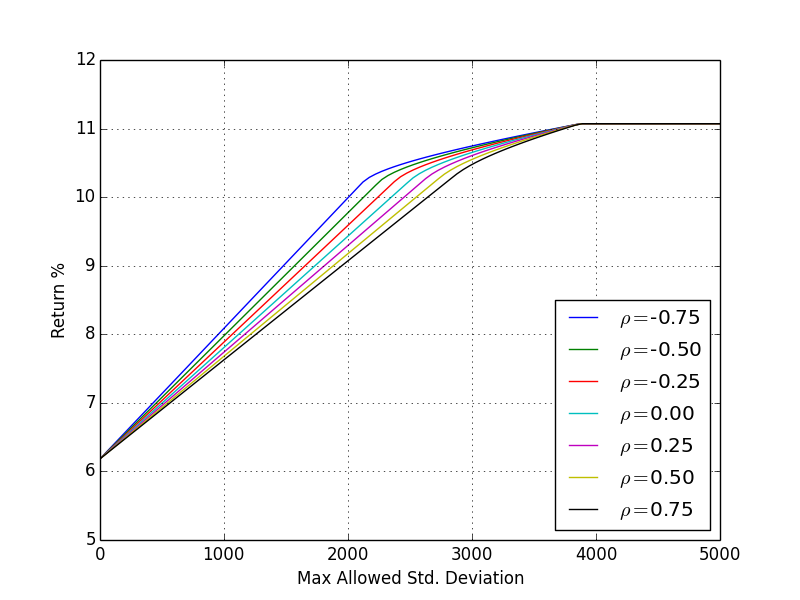
\includegraphics[scale=0.5]{markowitz.png}
\caption{Efficient frontiers based on the Markowitz model. The different curves correspond to different correlations between the stock returns.  Code is attached. The two files are ``plot\_markowitz\_efficient\_frontier.py'' and ``markowitz.py''. $\mu = (0.03, 0.035), \sigma=(0.1, 0.15), r = 0.02$.}
\label{fig:markowitz}
\end{figure}

\section{Average Value-at-Risk}
The Markowitz model involves a linear objective and a quadratic constraint. The objective is the expected return, and the constraint controls the variance of the return. The model can be switched around such that you specify the expected return you want, which leads to a linear constraint, and then you minimize the variance, which means you have a quadratic objective. Either way, there is a quadratic term.

Additionally, the Markowitz model discourages strategies that have high variance. This is a problem, because it penalizes low returns and high returns. Ideally, we would like to only penalize low returns.

Value-at-risk (V@R) controls the size of our losses. The $\text{V@R}_\alpha$ of a random variable $X$ is
\begin{equation*}
\text{V@R}(X) = \inf\{t : P(X \le t) \ge \alpha\}
\end{equation*}
Roughly speaking, average value-at-risk (AV@R) is a way to quantify the expected losses of a strategy. If $X$ is a continuous random variable, then the AV@R$_\alpha$ of a random variable X is defined as
\begin{equation*}
\text{AV@R}_\alpha (X) = \mathbb{E}[X | X \ge V@R(X)]
\end{equation*}
We can incorporate $AV@R$ into a stochastic program by using a set of linear constraints. Thus by using AV@R as our risk-measure, we can avoid quadratic terms in our portfolio optimization problem, plus it only penalizes losses.

Let's say there are two stocks and one risk-free asset. The risk-free asset's rate of return is 2\%. Also assume that the stock prices follow geometric Brownian motion and that the returns are not correlated. Thus
\begin{equation*}
dX_i(t) = \mu_i X_i(t) dt + \sigma_i dB_i(t)
\end{equation*}
where $i=1,2$. For stock $i$, $\mu_i$ is the average rate of return per year, and $\sigma_i^2$ the rate of return's variance per year.
Say we have \$10,000 to invest, and we want to maximum our returns after 3 years. Also suppose that
\begin{align*}
\mu &= (0.3, 0.035)\\
\sigma &= (0.1, 0.15)\\
\end{align*}
Let's say we could tolerate losing \$1,000. Let $x$ be vector representing the amount of money invested in each of the assets. $x_1$ and $x_2$ are for stocks 1 and 2, and $x_3$ is for the risk-free asset. Then we would like to solve
\begin{align*}
&\max_x \sum_{i=1}^2\mathbb{E}[e^{3\mu_i}]x_i + e^{0.02(3)}x_3 \text{ s.t.}\\
&\sum_{i=1}^3 x_i = 10,000\\
&\text{AV@R}_{0.05}\left(10,000 - \sum_{i=1}^2 X_i(3) X(0)^{-1} x_i + e^{0.02(3)} x_3\right) \le 1,000\\
&x \ge 0
\end{align*}
The term in the parentheses of $\text{AV@R}_{0.05}$ represents the random loss. If we discretize $X_i$ by choosing a bunch of scenarios, then we can turn the last constraint into a set of linear constraints. There will be an extra constraint and variable for each scenario. Discretizing $X_i(3)$ is fairly straightforward, because we know that it is log-normally distributed. We can also handle correlated returns. Section \ref{corr_gmb} shows how to correlate the stock returns. 

If we discretize $X_i(3)$ by drawing $N$ random variables for each stock, then the problem becomes
\begin{align*}
&\max_{x,w,\gamma} \sum_{i=1}^2 \bar{\mu}_i x_i +  e^{0.02(3)} x_3 \text{ s.t.}\\
&\sum_{i=1}^3 x_i = 10,000,  \forall k = 1,\ldots, N\\
& w_k \ge 10,000 - \sum_{i=1}^2 X^k_i(3) X(0)^{-1} x_i - e^{0.02(3)} x_3 - \gamma, \forall k = 1,\ldots, N\\
&x \ge 0, w \ge 0, \gamma \in \mathbb{R}
\end{align*}
where $\bar{\mu}_i = \frac{1}{N} \sum_{k=1}^N X_i^k(3)$.
It might not necessary to discretize the above problem, but it allows for more flexibility. We can make the model more complex, and then it's straightforward to add random events that affect the prices. Note that we need to decide how to invest our money at year 0, and then we sell it all at year 3. I wrote Python code that implements a Gurobi model for the above problem (``single\_stage.py''). It plots the efficient frontier (figure \ref{fig:single_stage}), which means that it specifies a maximum AV@R, and then maximizes the return.
\begin{figure}
\centering
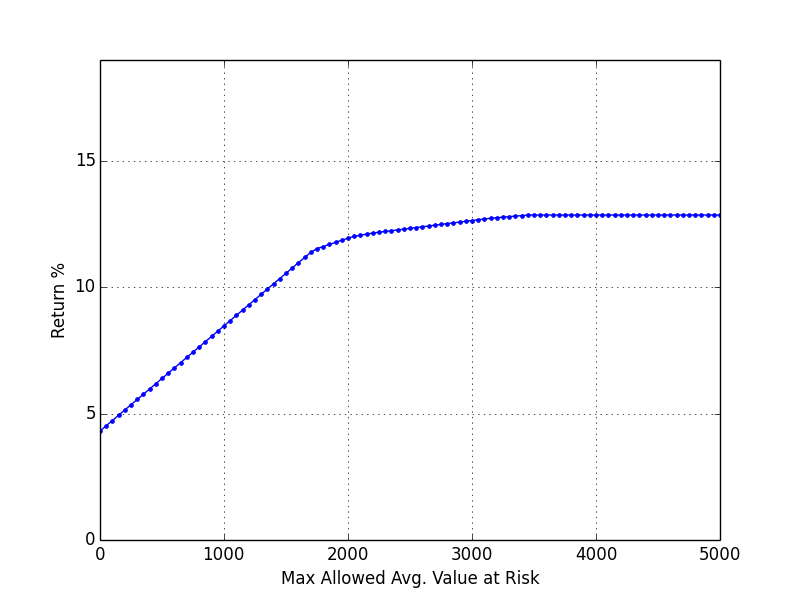
\includegraphics[scale=0.5]{single_stage.png}
\caption{Efficient frontier based on the single-stage AV@R model.  Code is attached (``single\_stage.py'').}
\label{fig:single_stage}
\end{figure}

\section{Multistage Portfolio Optimization Without Transaction Costs}
We might want to extend the model, and allow for asset reallocation at specified times. We will not include transaction costs, but we will include the possibility of correlated stock returns. Instead of just having $N$ scenarios, the plan is to use a scenario tree. Let's say we are allowed to reallocate our capital after the first year, and then we sell everything after year 3. We also have the same AV@R constraint as before, which, roughly speaking, limits our worst losses to be less than \$1,000.  The optimization problem is basically the same as the earlier one, but now we need to add another constraint. This constraint makes sure that we only allocate capital that we already have at each stage. Let $x^j$ be the allocation as of year $j$, then the problem becomes
\begin{align*}
&\max_{x,w,\gamma} \frac{1}{N}\sum_{k=1}^N\left[\sum_{i=1}^2 \bar{\mu}^k_i x^{2,k}_i +  e^{0.02(3)} x_3^{2,k}\right] \text{ s.t.}\\
&\sum_{i=1}^3 x_i^{j,k} = 10,000, j=1,2, \forall k=1,\ldots,N\\
& w_k \ge 10,000 - \sum_{i=1}^2 X_i^k(3) X(0)^{-1} x^{2,k}_i - e^{0.02(3)} x_3^{2,k} - \gamma, \forall k = 1,\ldots, N\\
&\sum_{i=1}^2 X_i^k(j) (x_i^{j+1,k}-x_i^{a(j+1,k)}) + e^{0.02j}(x_3^{j+1,k}-x_3^{a(j+1,k)}) = 0\\
&x \ge 0, w \ge 0, \gamma \in \mathbb{R}
\end{align*}

$a(j+1,k)$ means the ancestor of the node $(j+1,k)$. This notation is terribly confusing, but all I'm trying to denote with the $4^{th}$ line is that the amount of capital we have at each stage is equal to the amount we started with, plus the amount we made up to that point. We do not allow for extra capital to be injected at any stage.

Note that $x^{j+1}$ can depend on $X(j)$. In other words, we are allowed to adjust our reallocation based on the returns in year 1. I wrote Python code that creates a Gurobi model for this problem (``multi\_stage.py''). It then plots the efficient frontiers for different correlations between the stock returns (figure \ref{fig:multi_stage_no_transaction_costs}) (``plot\_efficient\_frontier\_for\_correlated\_returns.py'') . Since the size of the scenario tree is the number of branches cubed (3 stages), the number of branches at each node can't be too large. Thus computed many efficient frontiers for each correlation, and averaged them. This overestimates the expected return, but it seems to give a better picture than just maximizing the size of the tree. I decided to use 60 branches at each node, and calculated each efficient frontier 150 times.
Just like with the Markowitz model, the efficient frontier decreases as the correlation increases. Once again makes sense, because we can diversify more of the risk away when the stock returns are negatively correlated.
\begin{figure}
\centering
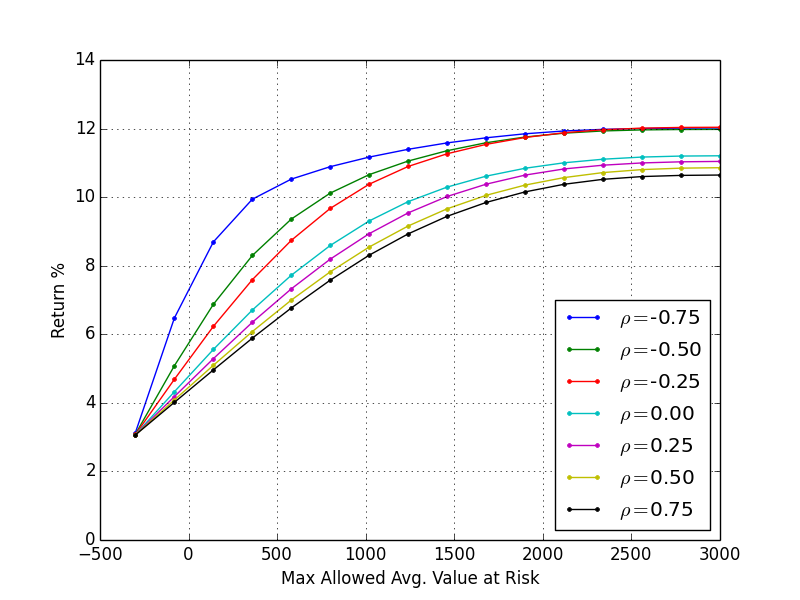
\includegraphics[scale=0.5]{multi_stage_no_transaction_costs.png}
\caption{Efficient frontier based on the multi-stage AV@R model. Does not include transaction costs.  Code is attached. There are two files: ``plot(...)returns.py'' and ``multi\_stage.py''.}
\label{fig:multi_stage_no_transaction_costs}
\end{figure}
\begin{figure}
\centering
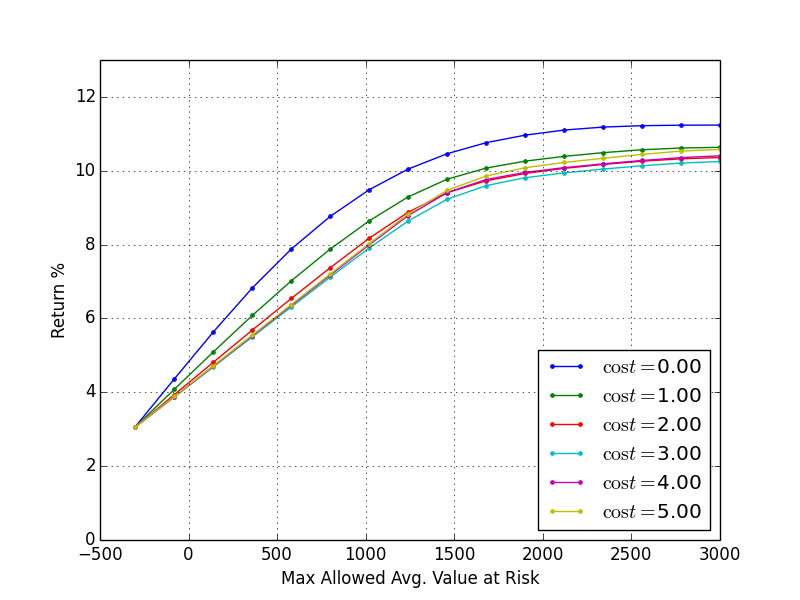
\includegraphics[scale=0.5]{multi_stage_with_transaction_costs.png}
\caption{Efficient frontier based on the multi-stage AV@R model. Does include transaction costs.  Code is attached.}
\label{fig:multi_stage_with_transaction_costs}
\end{figure}

\section{Multistage Portfolio Optimization With Transaction Costs}
Extending the above model to include transaction costs is relatively straightforward, because the units of $x$ is in the number of securities purchased. Thus we just need to keep track of the difference in the number of each type of stock and risk-free asset we own at each stage.

The model is the same as in the previous section. But now for all $i$ ($i$ denotes the security), we let
\begin{align*}
y_i \ge x_i^{2} - x_i^1\\
y_i  \ge x_i^{1} - x_i^{2}\\
y_i \ge 0
\end{align*}
There is a $y$ vector of variables at each node in the scenario tree at stage $j$. Let $c$ be the cost to trade one security. Then the objective is
\begin{equation*}
\max_{x,w,\gamma,y} \frac{1}{N}\sum_{k=1}^N\left[\sum_{i=1}^2 \bar{\mu}^k_i x^{2,k}_i +  e^{0.02(3)} x_3^{2,k}\right] - \frac{\text{cost}}{\text{number of nodes -1}}\sum_{\text{all } y} y\\
\end{equation*}
In words, the objective just now subtracts the cost of all the transactions. Together the constraint and objective  force $y$ to be equal to number of shares bought or sold. The reason we divide $c$ by $(\text{number of nodes}- 1)$ is that there is a vector of $y$ variables at every node in the tree except for at the root node. We just assume that we can buy the securities at the beginning without paying any transaction costs. As we would expect, the efficient frontier decreases as the costs go up (figure \ref{fig:multi_stage_with_transaction_costs}). As the transaction costs go up, the efficient frontier should be the same as the single-stage frontier. The increased costs discourage any trading after the beginning.

\bibliography{719_project.bib}
\bibliographystyle{ieeetr}

\end{document}

